\documentclass{article}
\usepackage[utf8]{inputenc}
\usepackage{graphicx}
\graphicspath{ {./images/} }
\usepackage{geometry}
 \geometry{
 a4paper,
 total={210mm,297mm},
 left=20mm,
 right=20mm,
 top=20mm,
 bottom=20mm,
 }

\title{384.178 SoC Design Lab}
\author{Aspodinger Daniel, Himler Patrick, Unfried Paul, Vogl Lukas }
\date{October 2020}

\begin{document}

\maketitle

\section{Abstract}

As a part of the course System on Chip (SoC) laboratory at the Technical Univerisity of Vienna, we want work on run time module power monitoring for Field Programmable Gate Array (FPGA) applications. Because power efficiency has become a major concern for all electronic devices, including FPGA, there is a need for accurate power monitoring without large overhead and performance losses. Our general approach is that the switching activity of the transistors at the hardware level and the overall power consumption are correlated. The main challenge for us is to identify those correlations. As an application we choose an Encryption/Decryption module which we want to implement on a Digilent ZedBoard Znyq-7000 Development Board. Later the question will arise if there is a systematic and generic method for monitoring of the power consumption during run time based on our implementation.

\section{Hierarchy chart}

The team consists of 4 members. Due the current situation we all work remote. Our joint work will be shared on Github. As we have a equally knowledge level of FPGA and VHDL the delimited work areas will maybe change during the duration of the project. For now Vogl Lukas and Patrick Himler will work on the implementation of the Encryption/Decryption module and Unfried Paul and Aspodinger Daniel will work on the power monitoring module.


\begin{figure}[h]
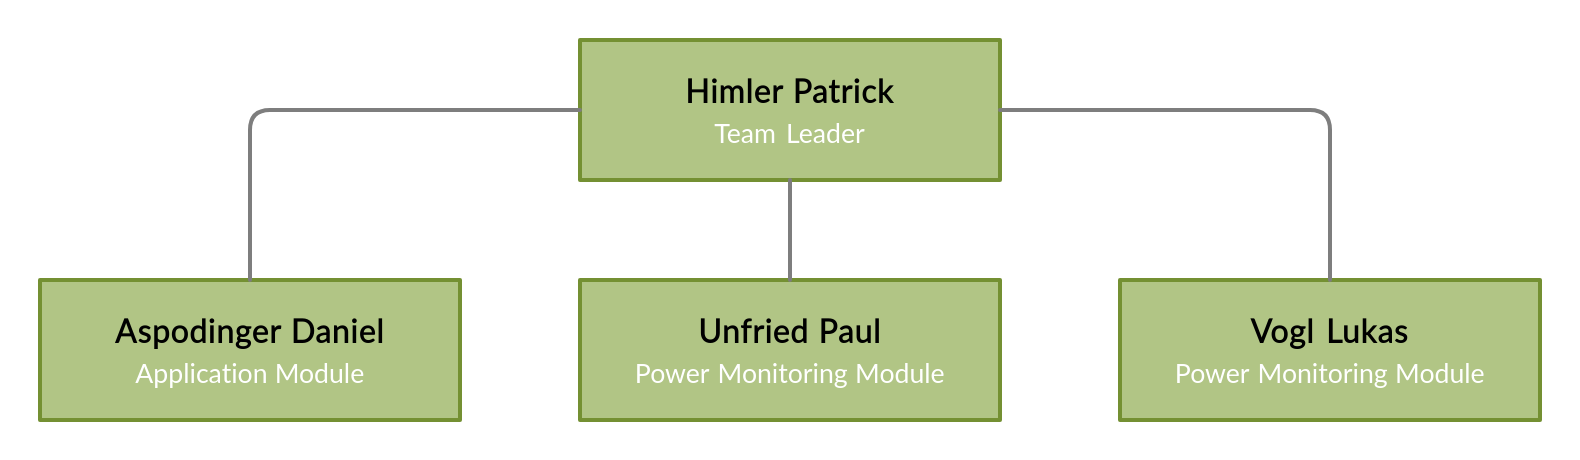
\includegraphics[width=17cm]{images/Hierachy chart.png}
\centering
\end{figure}

\end{document}
 
